
\section{Energieleitungen}
\label{section:antennen_energieleitungen}
\begin{frame}%STARTCONTENT

\begin{columns}
    \begin{column}{0.48\textwidth}
    
\begin{figure}
    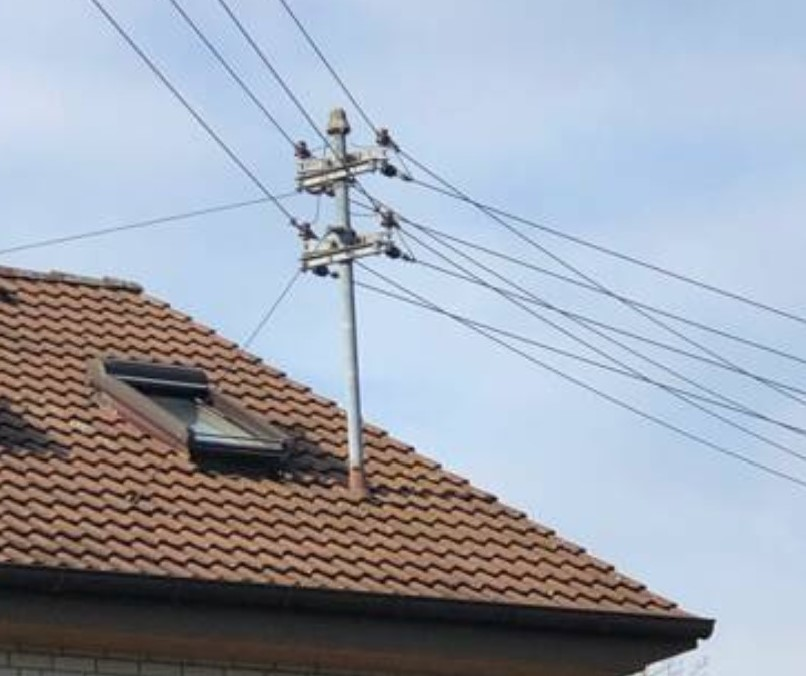
\includegraphics[width=0.85\textwidth]{foto/82}
    \caption{\scriptsize Dachständer}
    \label{n_Dachstaender}
\end{figure}

    \end{column}
   \begin{column}{0.48\textwidth}
       \begin{itemize}
  \item Antenne freihalten von Energieleitungen
  \item Bei Beschädigung der Antenne dürfen keine Teile und Leitungen die Energieversorungsleitungen berühren
  \end{itemize}

   \end{column}
\end{columns}

\end{frame}

\begin{frame}
\frametitle{Achtung}
Wenn eine Antenne eine Energieversorgungsleitung berührt,  besteht akute Gefahr von lebensgefährlichen Stromschlägen!

\end{frame}

\begin{frame}
\only<1>{
\begin{QQuestion}{NK311}{Was ist bei der Installation von Außenantennen insbesondere zu beachten?}{Zu benachbarten Energieversorgungsleitungen ist ein seitlicher Abstand von \qty{8}{\m} einzuhalten.}
{Für die Antenne muss eine Sturmversicherung abgeschlossen werden.}
{An der Antenne müssen die Kontaktdaten des Betreibers erkennbar angebracht sein.}
{Im Falle einer Beschädigung dürfen umstürzende oder herabfallende Teile und Leitungen keine Energieversorgungsleitungen berühren.}
\end{QQuestion}

}
\only<2>{
\begin{QQuestion}{NK311}{Was ist bei der Installation von Außenantennen insbesondere zu beachten?}{Zu benachbarten Energieversorgungsleitungen ist ein seitlicher Abstand von \qty{8}{\m} einzuhalten.}
{Für die Antenne muss eine Sturmversicherung abgeschlossen werden.}
{An der Antenne müssen die Kontaktdaten des Betreibers erkennbar angebracht sein.}
{\textbf{\textcolor{DARCgreen}{Im Falle einer Beschädigung dürfen umstürzende oder herabfallende Teile und Leitungen keine Energieversorgungsleitungen berühren.}}}
\end{QQuestion}

}
\end{frame}%ENDCONTENT
